% $Id%

% ++++++++++++++++++++++++++++++++++++++++++++++++++++++++++++++++++++++++++
%\pagebreak
\newpage
\enlargethispage{1cm}
\hypertarget{appendix-menutree}{}
\section{CrypTool Menus}
\label{s:appendix-menutree}

This appendix contains at the following page the complete menu tree of
CrypTool\index{CrypTool} version 1.4.30\footnote{%
  In parallel to CrypTool 1.x\index{CrypTool 1.x} the future versions
  CrypTool 2\index{CrypTool 2.0} and JCrypTool\index{JCrypTool 1.0}
  are currently developed in the CrypTool project.\\
  These future versions are currently (August 2009) beta versions, but they
  are stable enough to be used by end-users too. If the according release
  versions are available, we will add the appropriate menus and menu trees.\\
}. 

Which menu items in CrypTool are active (that means not greyed), depends on
the type of the currently active document window.

The brute-force analysis\index{Attack!brute-force} for DES e.~g. is only
available, if the active window is opened in the hexadecimal view. 
On the other hand the menu item ``Generate Random Numbers\dots''
is always available (even if no document is opened).

%The following four types of documents exist in CrypTool:
%\begin{center}
%\begin{tabular}{rl}
%\bf Code letter & \bf Type of document \\
%T & Text file view\\
%H & Hexadecimal view\\
%P & Diagram/plot view (histogram, autocorrelation)\\
%O & OpenGL graphics view\\
%\end{tabular}
%\end{center}


%\nobreak
\clearpage
\begin{figure}[hb]
\begin{center}
\vspace{-30pt}
%\frame{  %TeX macht einen Rahmen (siehe viewport) drumherum -- gut zum Testen
%\includegraphics[scale=0.25, angle=270, viewport=200 30 2660 1430]
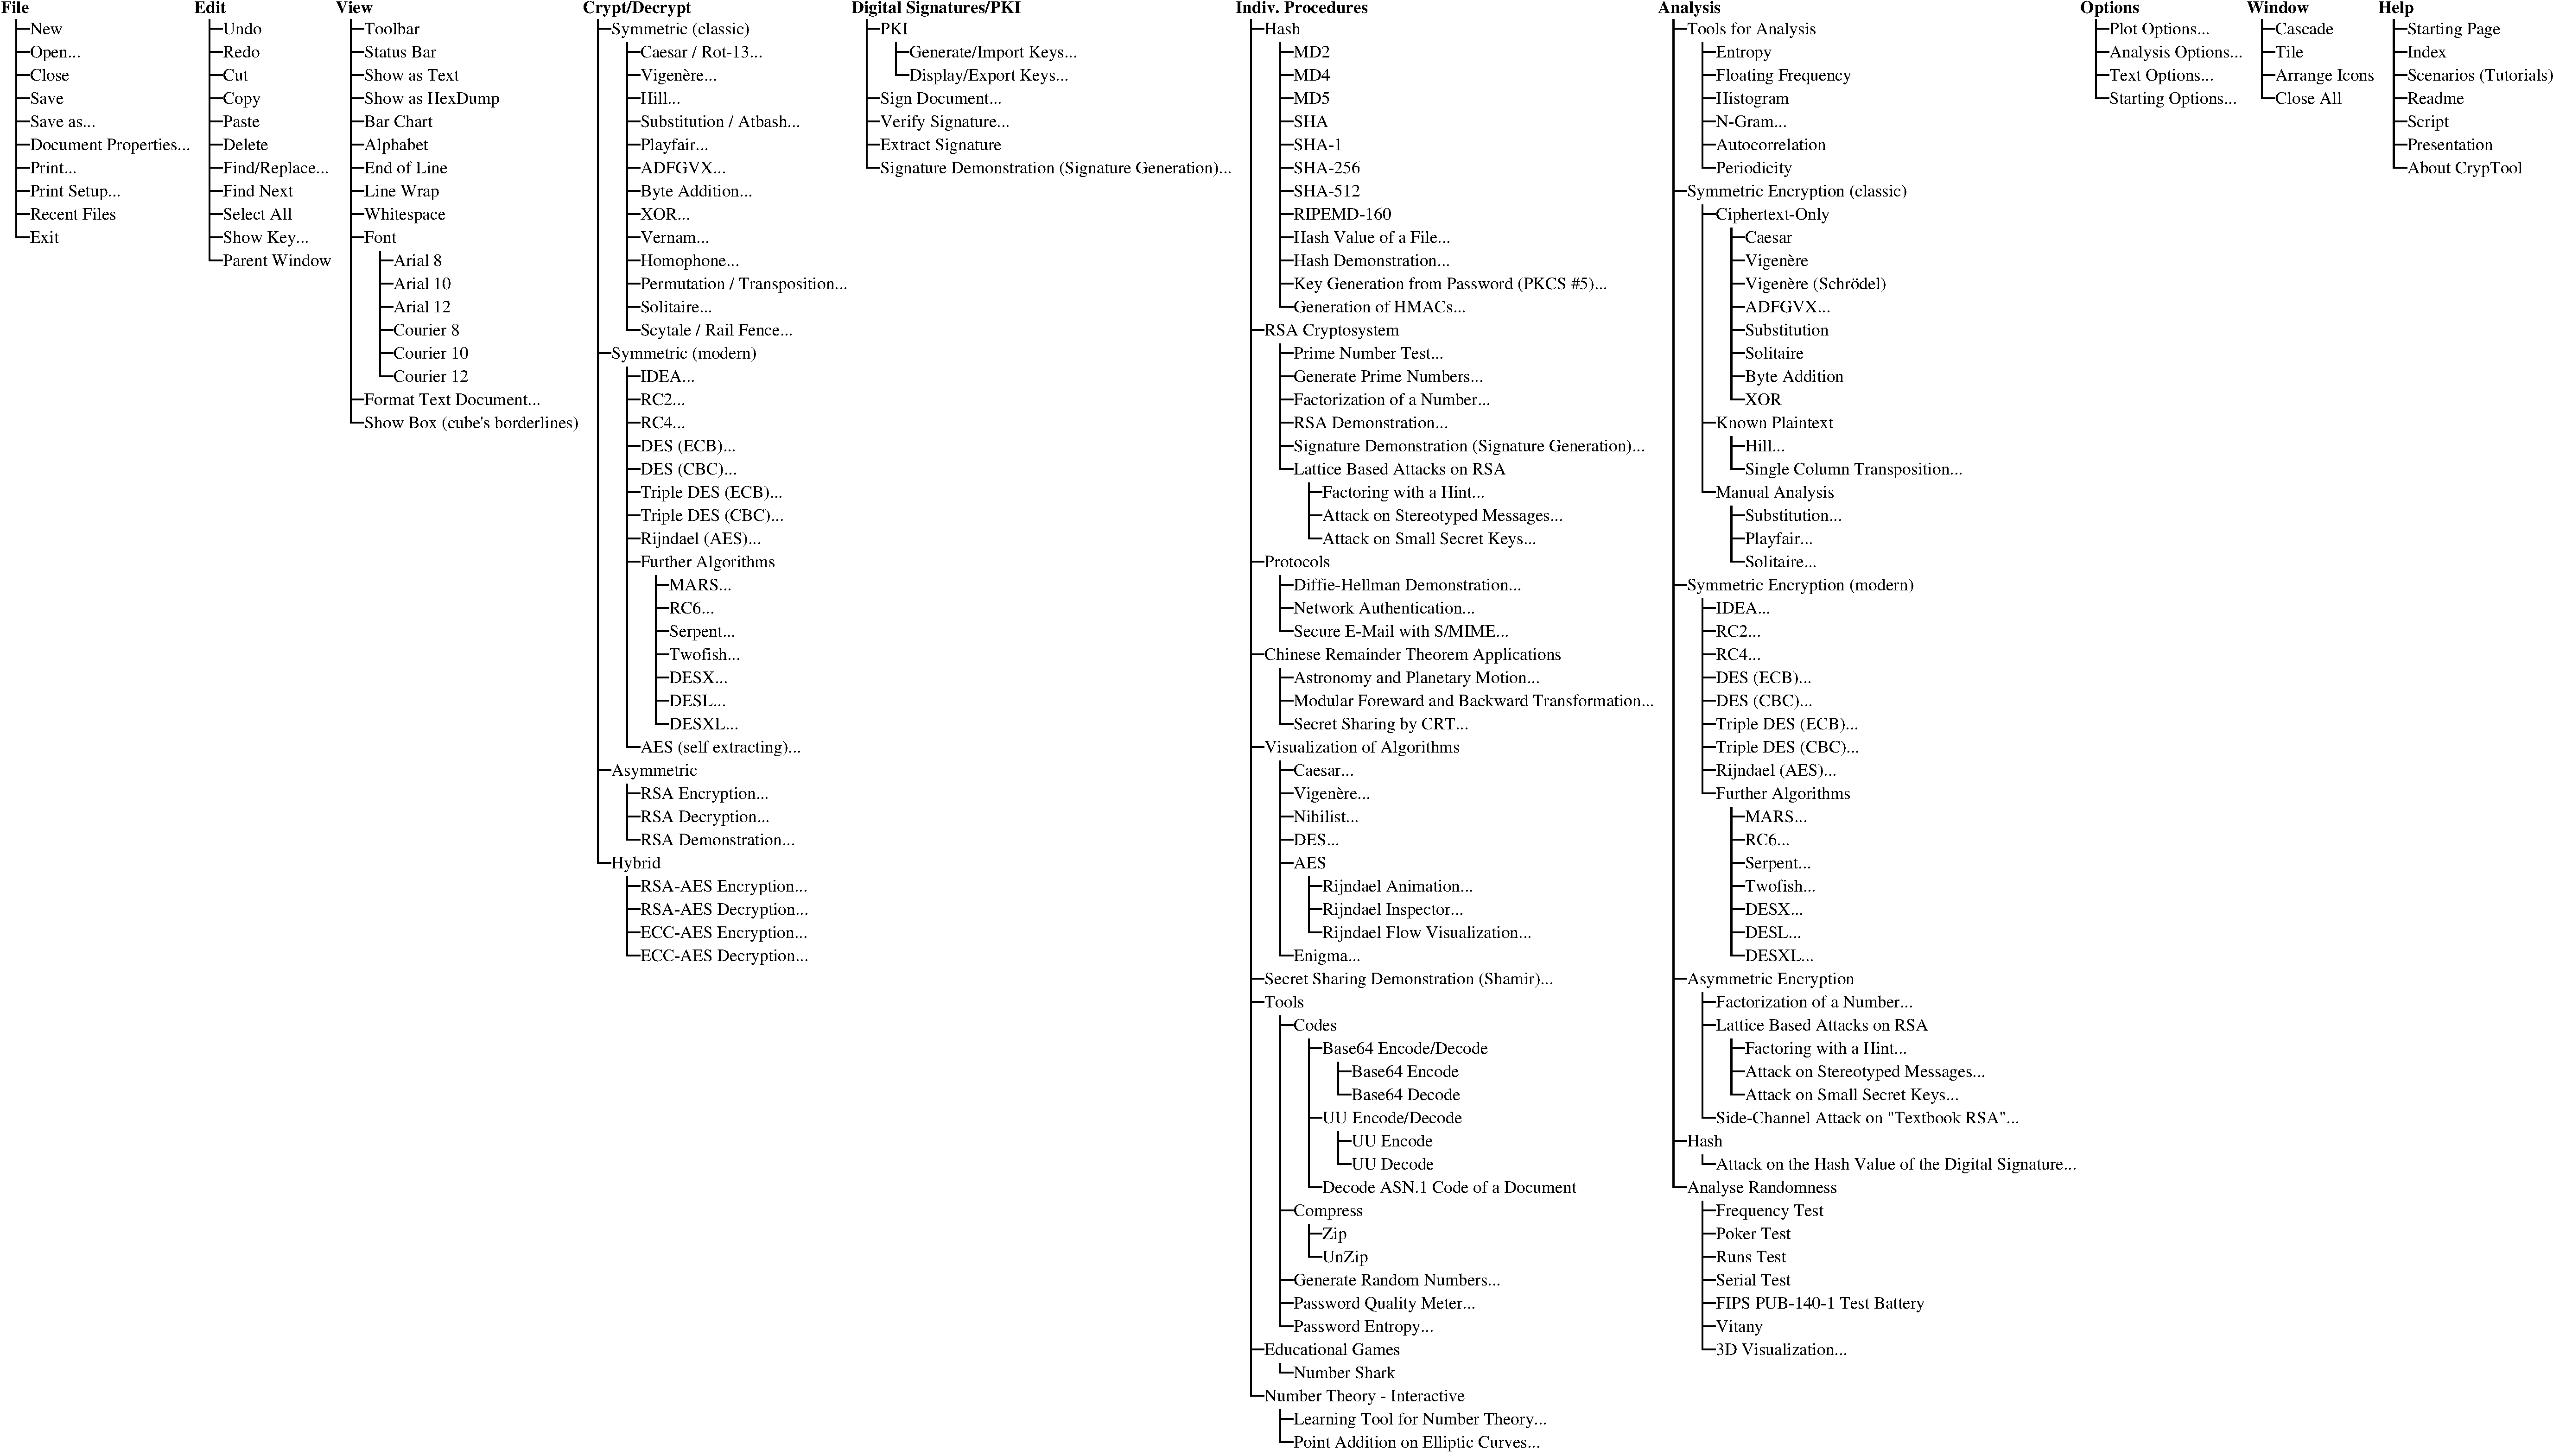
\includegraphics[scale=0.25, angle=270]
                {figures/cryptool-menu-en}
%viewport=rand-links? rand-unten breite hoehe? [bezogen auf querformat]
%}
\caption{Complete overview of the menu tree of CrypTool 1.4.30} 
\label{menuoverview}
\end{center}
\end{figure}
\clearpage
